\section{Introduction}\label{SEC:introdcution}
\subsection{Contexte général}
Dans de nombreux domaines, l’imagerie constitue un moyen efficace d’acquérir et d’agréger rapidement un volume d’informations considérable, indispensable à la prise de décision. À titre d’exemple, les applications de suivi des changements exploitent des techniques d’imagerie afin de cartographier et d’évaluer les impacts d’une catastrophe naturelle sur une zone sinistrée. 

Pour l’acquisition d’images, plusieurs types de capteurs peuvent être employés. De manière intuitive, l’on pense aux capteurs photographiques, capables de détecter les ondes électromagnétiques des domaines ultraviolet, visible et infrarouge. Toutefois, ces dispositifs présentent une limitation majeure : ils ne permettent pas l’imagerie en toutes conditions, leur fonctionnement étant fortement dépendant de l’éclairement et des conditions atmosphériques. 

Afin de pallier cette limitation, la Royal Air Force développa, au cours de la Seconde Guerre mondiale, le premier radar aéroporté capable de produire une image radar analogique : le H2S. Ce système permit aux forces britanniques d’améliorer la précision de leurs bombardements nocturnes en détectant les reliefs et les zones urbaines, dont la représentation était affichée sur un écran cathodique. 

À la fin des années 1940, de nouvelles avancées dans les technologies d’imagerie radar furent réalisées, parmi lesquelles le radar à fauchée latérale. Ce dispositif consiste à orienter une antenne latéralement afin de capturer l’image d’une bande étendue du sol. Les premiers systèmes SLAR\footnote{Side Looking Airborn Radar ou radar à fauchée latérale} fonctionnels furent testés au début des années 1950 et, à la fin de la décennie, les premières cartes radar continues du terrain purent être produites.

\begin{figure}[ht]
    \begin{minipage}[t]{0.45\textwidth}
        \centering
        \vspace{0pt}
        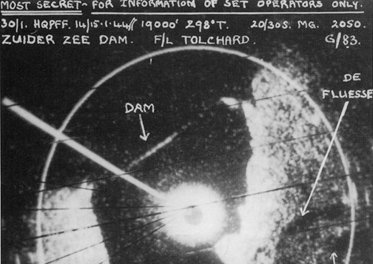
\includegraphics[width=0.9\linewidth]{src/biblio_sar/img/H2S_zuider_zee.jpg}
        \caption{Image du radar H2S réalisée au dessus de la Zuider Zee aux Pays-Bas \cite{h2s_source}}
        \label{fig:h2s_zuider_zee}
    \end{minipage}
    \hfill
    \begin{minipage}[t]{0.45\textwidth}
        \centering
        \vspace{0pt}
        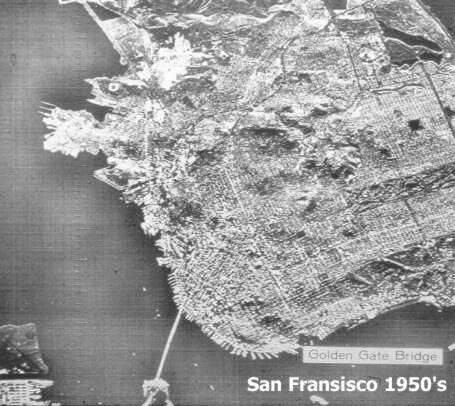
\includegraphics[width=0.9\linewidth]{src/biblio_sar/img/first_SLAR_image.png}
        \caption{Une des premières image d'un radar à ouverture réelle acquise par un radar à fauchée latérale \cite{colin_radar_images}}
        \label{fig:first_slar_image}
    \end{minipage}
\end{figure} 


Ainsi, l’imagerie radar revêt un intérêt manifeste tant dans le domaine civil que militaire. Elle se distingue notamment par sa capacité d’observation en toutes conditions météorologiques et à tout moment, garantissant une continuité d’acquisition que ne permettent pas les systèmes optiques. Par ailleurs, les propriétés propres à la technologie radar confèrent des possibilités d’analyse spécifiques. L’interférométrie des signaux, exploitant à la fois l’amplitude et la phase, permet notamment d’estimer des altitudes avec une grande précision. En outre, la complémentarité avec l’imagerie optique est particulièrement remarquable : tandis que cette dernière met en évidence les caractéristiques physico-chimiques des surfaces observées, l’imagerie radar est sensible aux propriétés géométriques des cibles, à la nature des matériaux ainsi qu’à leur état. Ces paramètres, essentiels à de nombreuses applications, demeurent souvent inaccessibles par les moyens optiques traditionnels. 

\subsection{Motivation d'un radar à synthèse d'ouverture}

Bien que l’imagerie radar conventionnelle soit performante, elle présente une limite majeure : la résolution. En effet, dans le cas d’un SLAR/RAR\footnote{Real Aperture Radar ou radar à ouverture réelle}, la résolution en azimut, qui correspond à la taille de la tache au sol, s'exprime de la manière suivante \cite{radartutorial} :

\begin{equation}
\delta_{az} = \frac{h\times\lambda}{L\times \cos{\theta}}
\end{equation}
Où :
\begin{description}
    \item[$\delta_{az}$] : est la résolution en azimut [m]
    \item[$h$] : est la hauteur de l'antenne par rapport au sol [m]
    \item[$\lambda$] : est la longueur d’onde [m]
    \item[$L$] : est la longueur physique de l’antenne [m]
    \item[$\theta$] : est l'angle d'incidence [°]
\end{description}

Cette relation montre qu’une résolution azimutale élevée nécessite une antenne de très grande dimension. Or, dans la pratique, les contraintes liées à la capacité d’emport des vecteurs aériens rendent cette solution peu réaliste. Ainsi, les radars à ouverture réelle (RAR) et à ouverture réelle latérale (SLAR) sont rapidement confrontés à des limites physiques qui restreignent fortement leurs performances. Leur résolution dépend directement de la taille de l’antenne et de la géométrie de visée : plus la distance entre le radar et la scène observée augmente, plus la résolution au sol se dégrade. Par conséquent, ces systèmes ne permettent pas d’obtenir des images suffisamment détaillées pour les besoins d’observation fine, ce qui limite leur emploi à des tâches de détection ou de surveillance globale où la précision spatiale n’est pas déterminante.

De nombreuses applications modernes d’imagerie radar ne peuvent donc pas être réalisées avec des systèmes RAR ou SLAR. La cartographie de haute résolution, la caractérisation des structures au sol, la génération de modèles numériques de terrain, ainsi que les techniques d’interférométrie et de polarimétrie exigent une stabilité de phase et une résolution métrique à submétrique qu’un radar à ouverture réelle ne peut atteindre. Le développement du radar à synthèse d’ouverture (SAR\footnote{Synthetic Aperture Radar ou radar à synthèse d'ouverture}) a précisément permis de dépasser ces limitations en reproduisant, par traitement du signal, l’effet d’une antenne de grande dimension, ouvrant ainsi la voie à l’imagerie détaillée depuis des plateformes aériennes et spatiales, pour des applications allant de la topographie à la surveillance environnementale.

\subsection{Positionnement}

Depuis le début des années 2010, le développement des drones de petite taille a connu une adoption à grande échelle pour des applications industrielles. Initialement utilisés à des fins militaires ou récréatives, ces systèmes ont rapidement trouvé leur place dans des secteurs tels que l’énergie, la construction, l’agriculture et la logistique, permettant la surveillance des infrastructures, la cartographie 3D et la gestion de sites sensibles. Cette évolution a été rendue possible grâce aux progrès technologiques — miniaturisation des capteurs, automatisation des vols, stabilisation des images et intégration de l’intelligence artificielle — qui ont transformé les drones en outils fiables et efficaces pour des missions industrielles complexes, complétant ainsi les capacités offertes par les radars aéroportés classiques \cite{wikipedia_drone,wikipedia_dji_matrice,foxtech_drone}.

L’évolution des plateformes légères permet désormais d’envisager l’embarquement de radars à synthèse d’ouverture (SAR) sur des drones, offrant la possibilité de réaliser des acquisitions d’images à haute résolution et des cartographies détaillées de zones ciblées. Dans ce contexte, le déploiement d’un essaim de drones apparaît comme une approche pertinente : chaque plateforme transporte une charge utile autonome intégrant le radar, laquelle assure la collecte et le stockage local des données. Le traitement et la fusion des informations sont réalisés après la mission, ce qui limite les contraintes liées aux communications en temps réel et simplifie la planification des opérations.

L’utilisation d’un essaim confère plusieurs avantages d’un point de vue opérationnel et scientifique. Elle permet de renforcer la résilience et la redondance dans la capture d’images, en particulier dans des environnements contestés, sinistrés ou difficilement accessibles. La conception de la charge utile constitue une étape préalable essentielle : la validation sur un drone unique permet ensuite d’envisager la réplication et la coordination au sein de l’essaim. Cette architecture soulève toutefois des problématiques techniques importantes, notamment en matière de multi-capteurs et de fusion de données, qui sont nécessaires pour obtenir des images radar fusionnées et cohérentes à partir des acquisitions dispersées.

Les applications de ce type de système sont à la fois civiles et stratégiques. Dans le domaine civil, elles contribuent à la surveillance des écosystèmes, à la prévention des risques naturels et à la production de données fiables pour l’aménagement du territoire et la gouvernance. Dans un contexte militaire ou stratégique, l’essaim permet une cartographie et une reconnaissance précises, même dans des zones hostiles ou couvertes, tout en garantissant une redondance et une adaptabilité accrues. Cette dualité illustre le potentiel des drones SAR en essaim comme outil pertinent à la fois pour la recherche, la gestion environnementale et la défense.

\newpage
1. Introduction

Contexte général : radar, observation tout temps, intérêt civil et militaire.

Besoin d’imagerie haute résolution → limites des radars conventionnels → motivation du SAR.

Positionnement spécifique : SAR embarqué sur drones, multi-capteurs, fusion et détection.

2. Principes de base du radar et du SAR

Rappels radar : portée, Doppler, résolution, SNR.

Limites des radars conventionnels pour l’imagerie.
speckle (chatoiement) 

Principe du SAR : ouverture synthétique, compression en distance et en azimut.

3. Algorithmes de traitement SAR (formation d’image)
3.1 Compression en distance et en azimut
3.2 Algorithmes classiques

Range-Doppler

Chirp Scaling

omega–k (Range Migration Algorithm)

Backprojection

3.3 Limitations et hypothèses

Trajectoire rectiligne idéale, scène plane, hypothèse cible ponctuelle.

Contraintes en bande, navigation et coût calcul.

3.4 Comparaison des algorithmes
4. Avancées récentes en traitement SAR

Compensation de mouvement (MOCO), autofocus.

Traitements temps-fréquence et robustes.

Implémentations temps réel (GPU, FPGA).

Approches émergentes (IA, deep learning pour focalisation).

5. SAR embarqué sur drones (UAV-SAR)
5.1 Intérêt et spécificités

Portabilité, observation basse altitude, flexibilité.

5.2 Contraintes UAV

Masse/énergie, vibrations, trajectoire non idéale, volume de données.

5.3 Travaux académiques (ex. Pelle 2020, projets universitaires)
5.4 Développements industriels (mini-SAR sur drones militaires et civils)
5.5 Algorithmes adaptés

Backprojection robuste, navigation assistée GNSS/IMU, correction post-traitement.

6. Fusion multi-drones et SAR collaboratif
6.1 Intérêt : couverture étendue, redondance, meilleure résolution.
6.2 Contraintes : synchronisation temporelle, cohérence de phase, calibration inter-capteurs.
6.3 Travaux existants : MIMO-SAR, expériences UAV multi-capteurs.
6.4 Limites actuelles et défis pour l’avenir.
7. Détection en imagerie SAR
7.1 Objectif et enjeux de la détection

Cibles ponctuelles vs étendues, clutter, hétérogénéité du milieu.

7.2 Algorithmes classiques de détection

CFAR (CA-CFAR, OS-CFAR, GO-CFAR, SO-CFAR).

Détection par seuillage global et adaptatif.

7.3 Limites des méthodes classiques

Environnements hétérogènes, forte densité de clutter, faible SNR.

7.4 Approches avancées

Détection bayésienne et probabiliste.

Exploitation de l’information polarimétrique/interférométrique.

Apprentissage automatique (SVM, réseaux de neurones).

Deep learning pour la détection et classification d’objets dans les images SAR.

7.5 Évaluation des performances

Probabilité de détection (Pd), taux de fausses alarmes (Pfa).

Jeux de données et benchmarks (MSTAR, OpenSAR, etc.).

8. Discussion et perspectives

Comparaison des approches (formation image vs exploitation).

Verrous scientifiques actuels : navigation précise, traitement distribué, robustesse en clutter.

Perspectives : SAR multi-drones collaboratifs, IA pour fusion + détection en temps réel.

9. Conclusion

Synthèse des connaissances actuelles.

Positionnement de ton projet par rapport à l’état de l’art.